\section{Web Interface} \label{sec:web}
We use the Flask framework to build the web front end. We use the Flask framework to build the web front end. The user first goes to \lstinline{index.html}, then enters query and selects the search method. If the user want to use zone search, go to \lstinline{zone_search.html}, enter query and select the zone to search, as shown in Figure \ref{search-11}. The user's query and selected search method are passed to \lstinline{results.html} through a post request, the search is executed and the output is printed.
\begin{figure*}[h]
\centering
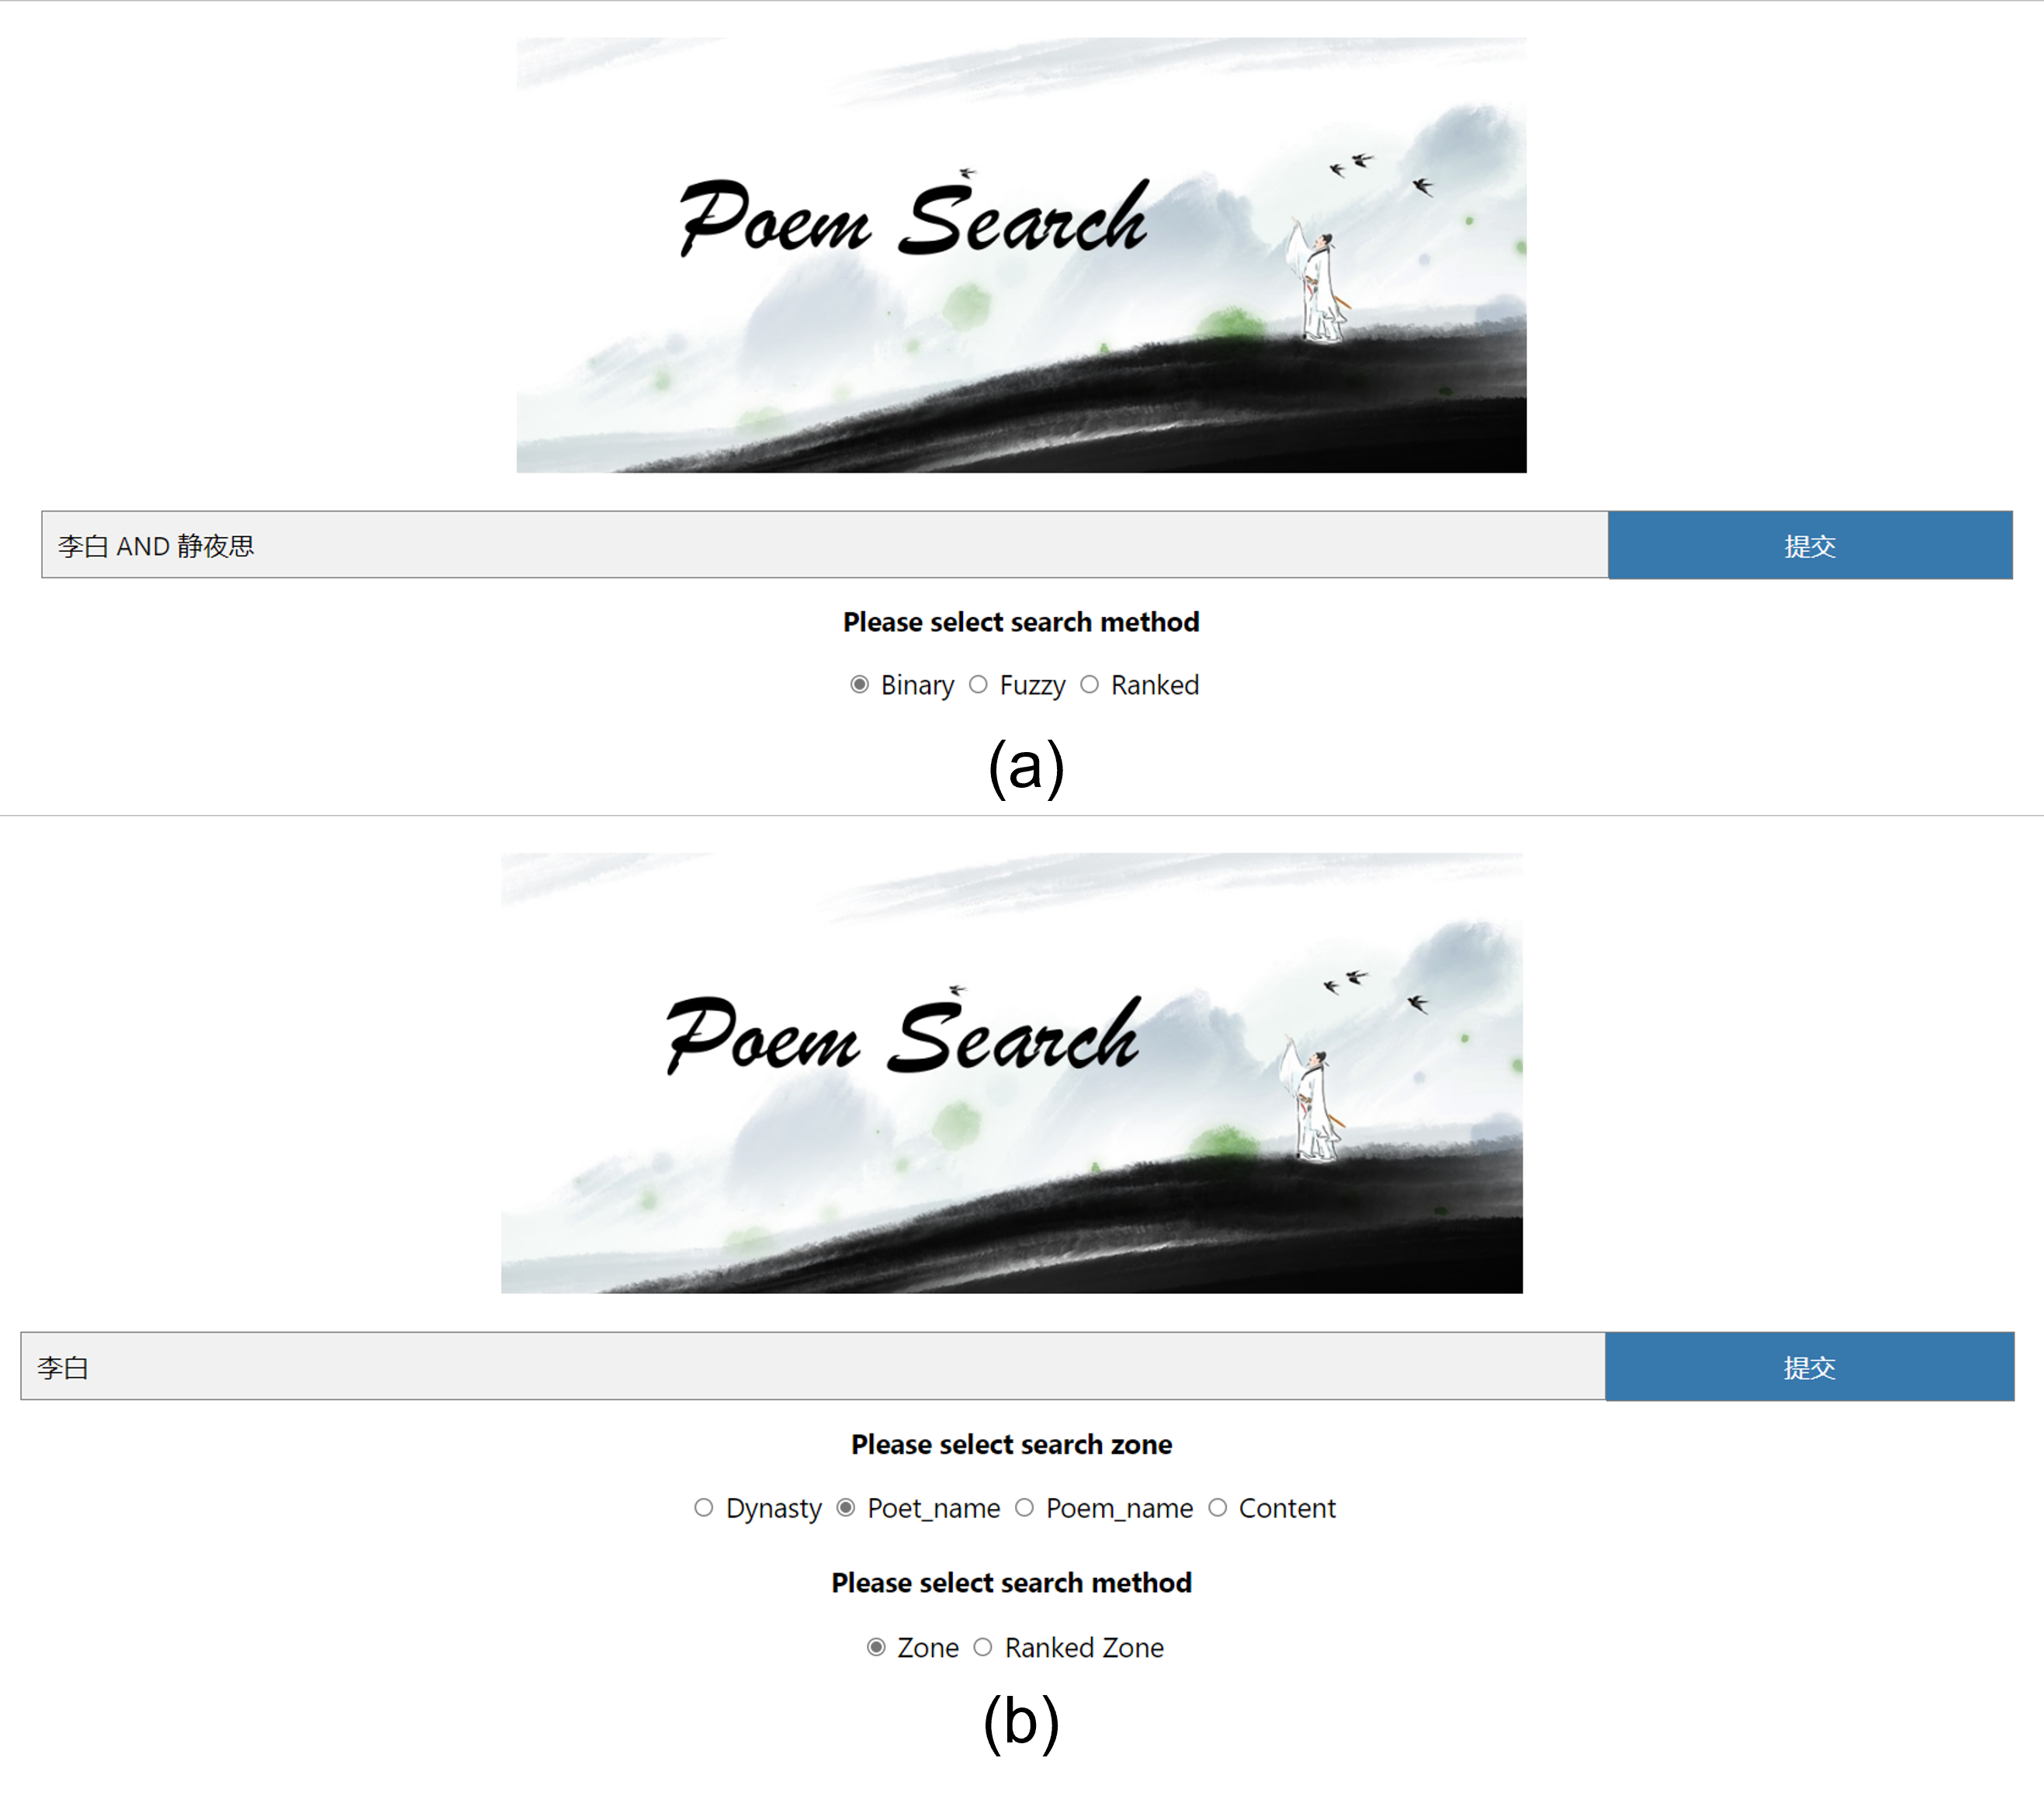
\includegraphics[width=0.7\textwidth]{figure/interface.png}
\caption{(a)\lstinline{index.html} (b)\lstinline{zone_search.html}}
\label{search-11}
\end{figure*}
For binary search, fuzzy search and ranked search, \lstinline{results.html} unpacks the form sent by the user through the request, and selects the corresponding search model to process the query according to the search method. Examples are shown in Figure \ref{search-9}.
\begin{figure*}[h]
\centering
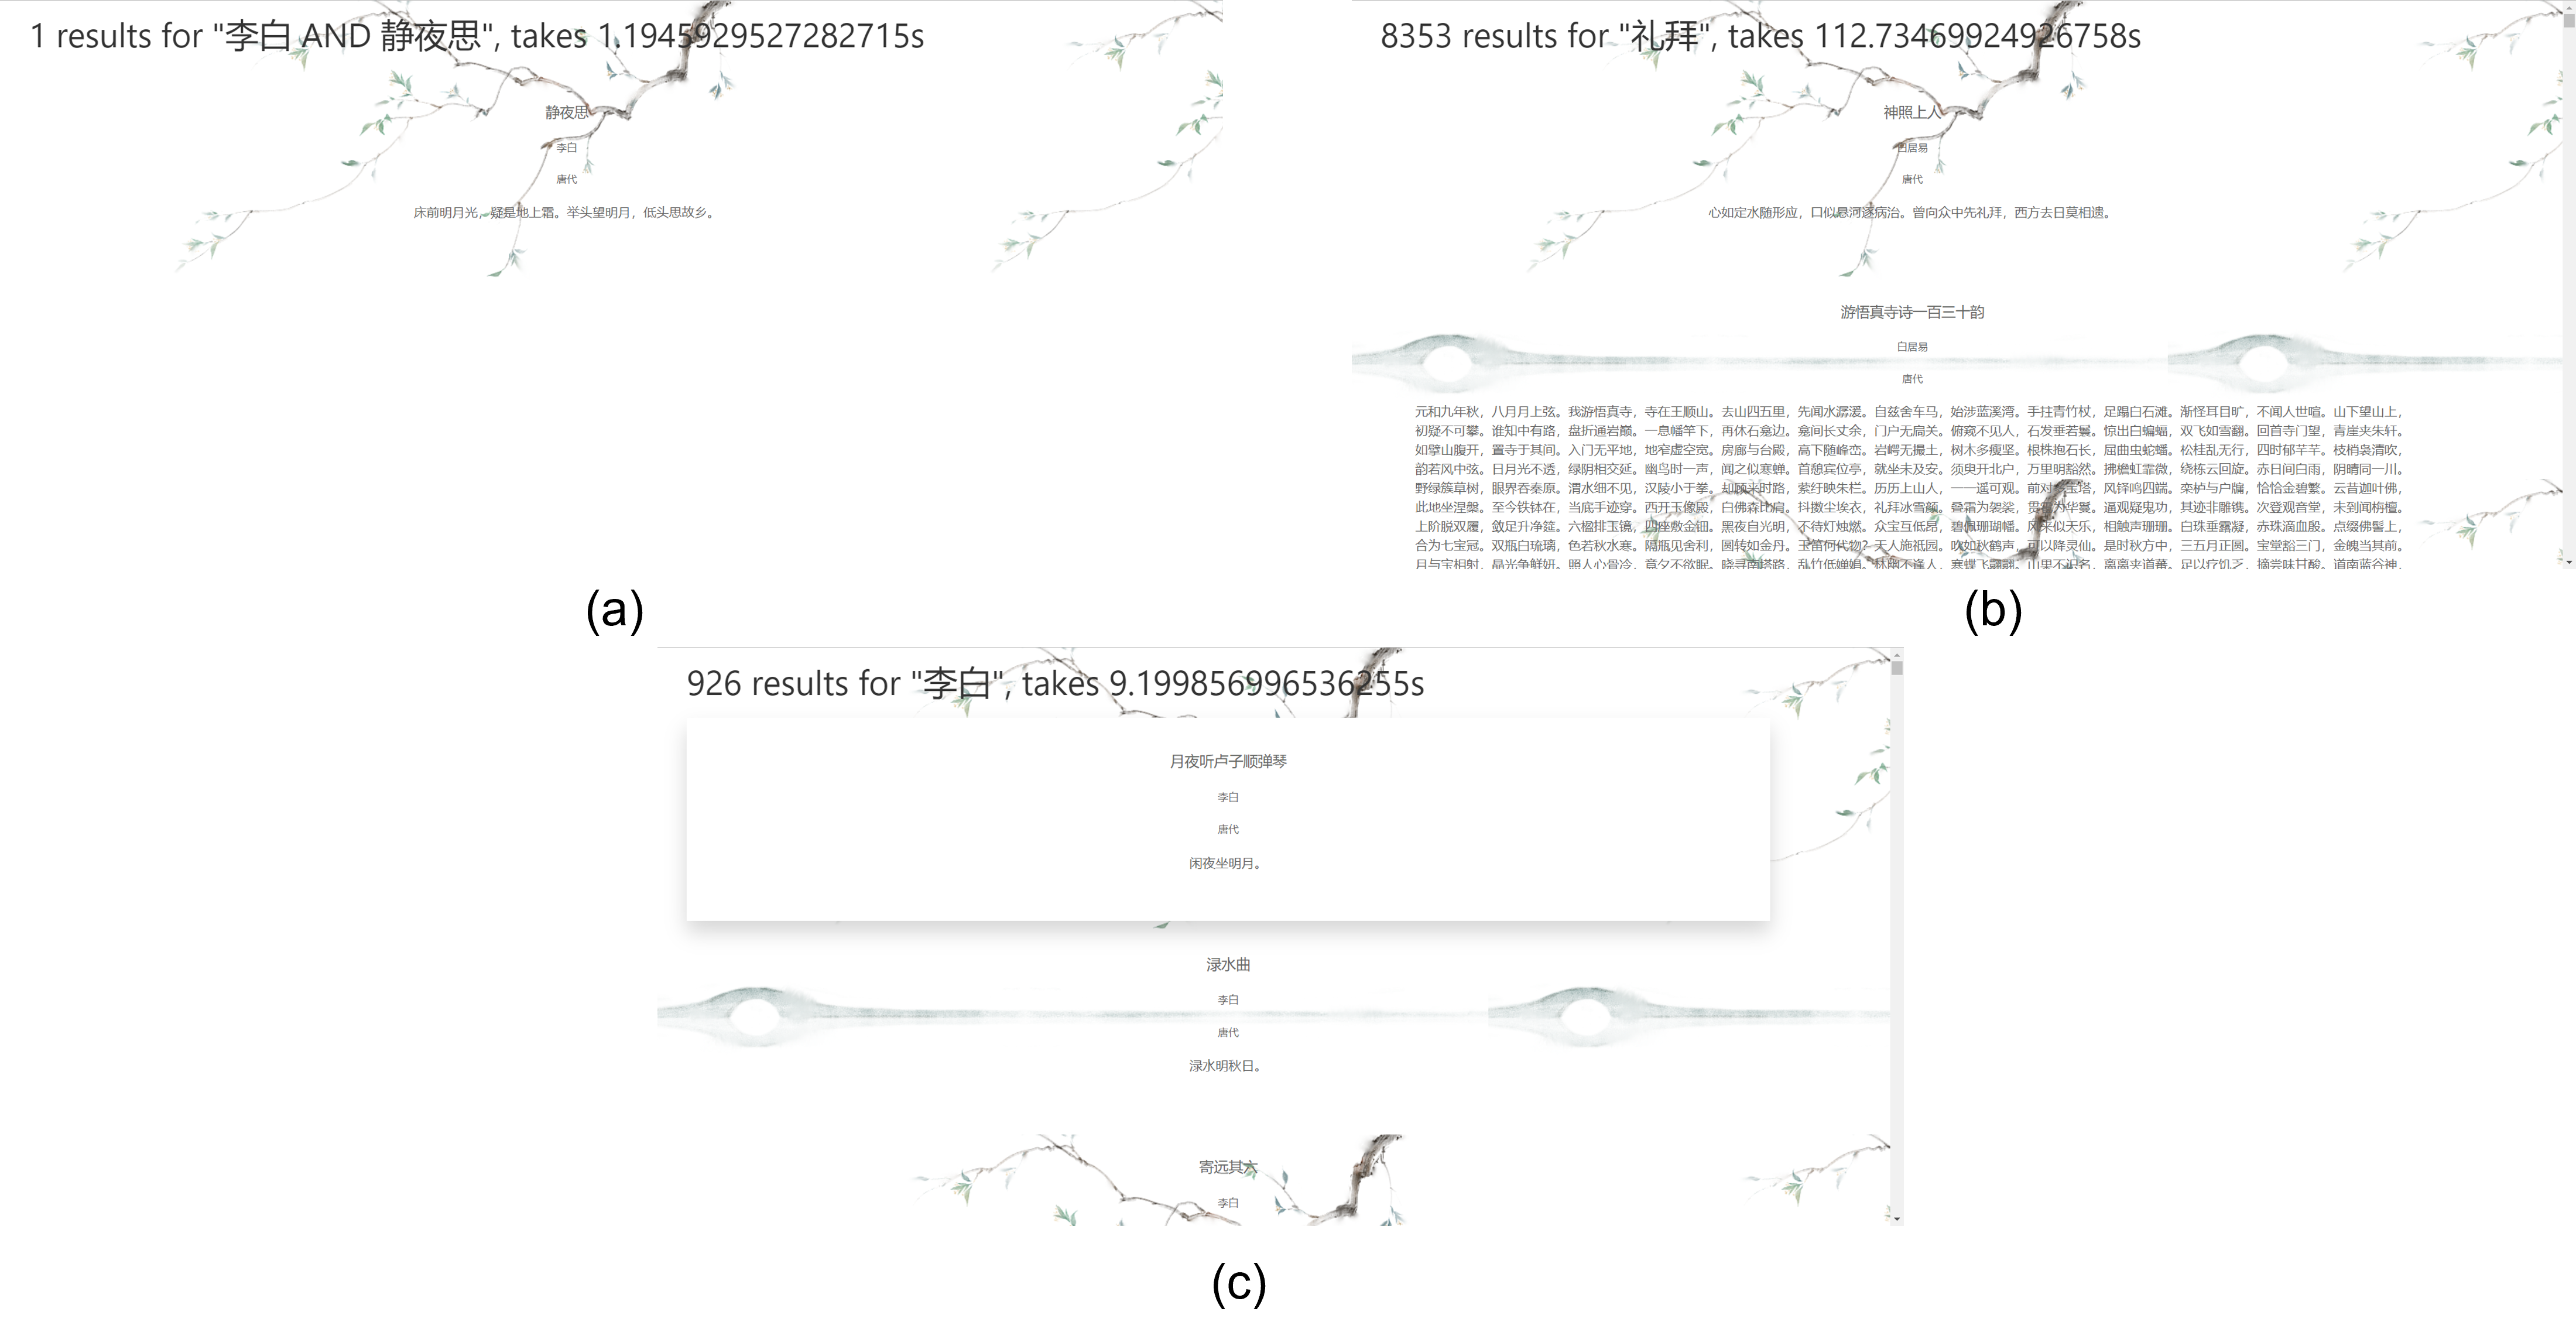
\includegraphics[width=0.7\textwidth]{figure/result1.png}
\caption{(a)\lstinline{Binary search} (b)\lstinline{Fuzzy search}(c)\lstinline{Ranked search}}
\label{search-9}
\end{figure*}

Similarly, for zone search, \lstinline{results.html} unpacks the form sent by the user through the request, selects the zone search search model according to the search method, and processes the query by dynasty, poet, poem name and content according to the corresponding zone, as shown in Figure \ref{search-10}. Show.

\begin{figure*}[h]
\centering
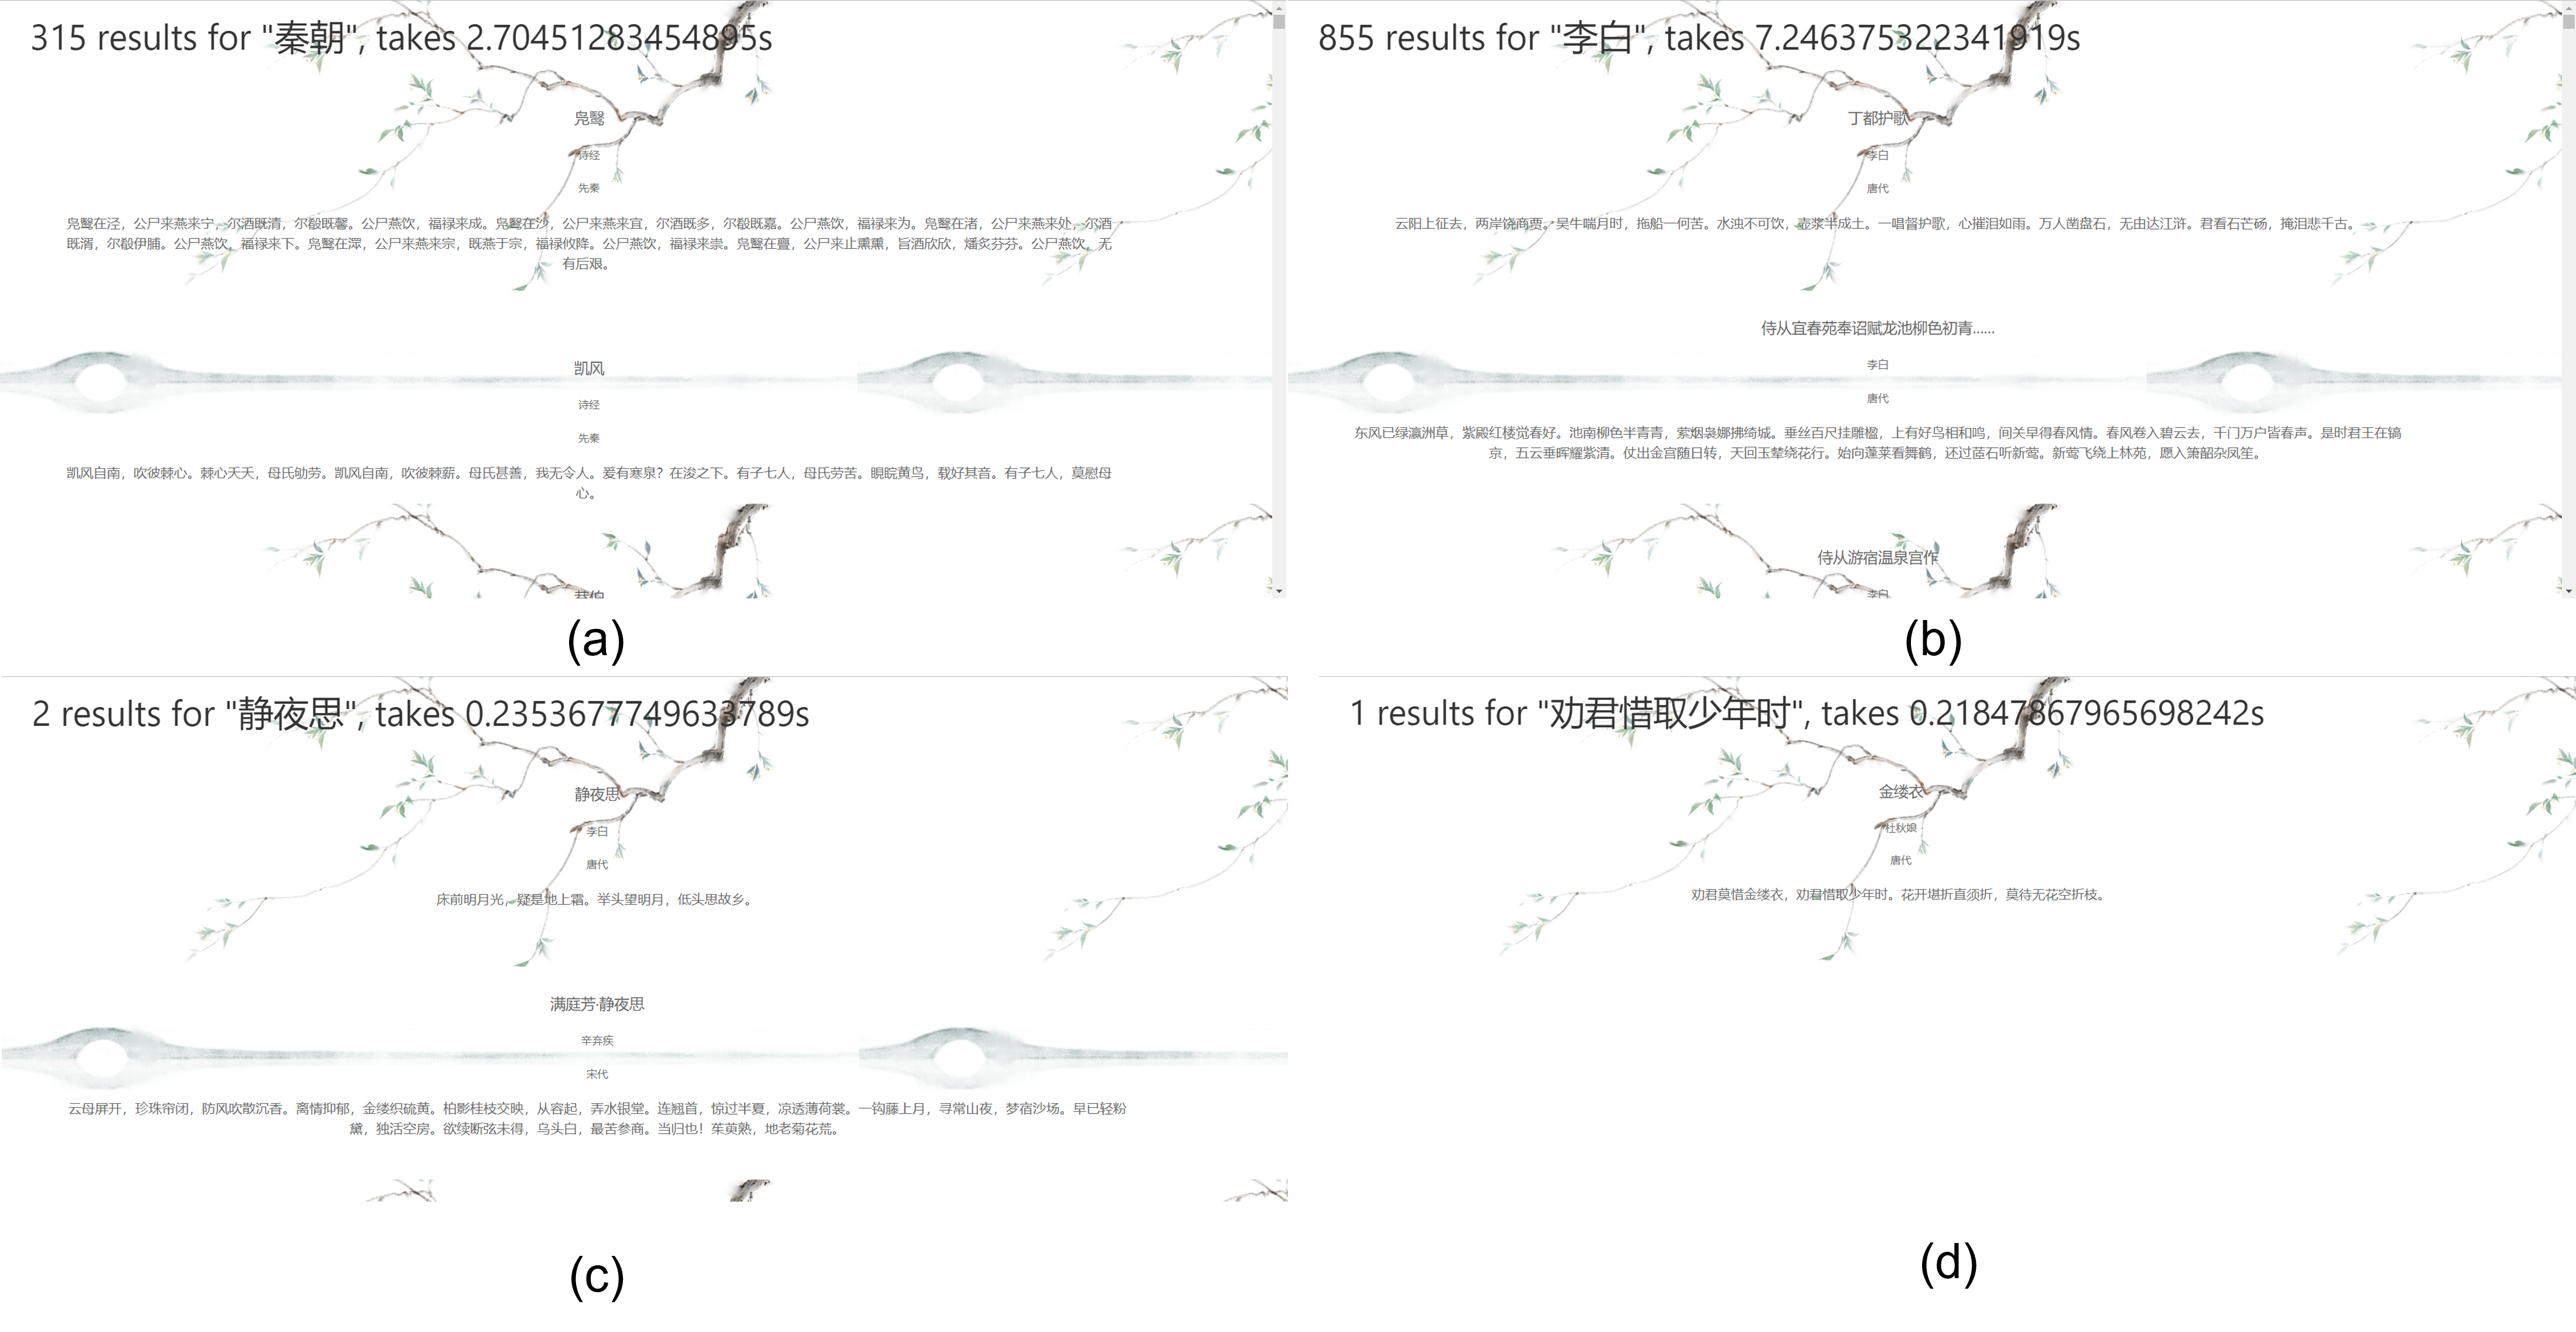
\includegraphics[width=0.7\textwidth]{figure/result2.png}
\caption{(a)\lstinline{zone search for dynasty} (b)\lstinline{zone search for poet}(c)\lstinline{zone search for poem}(d)\lstinline{zone search for content}}
\label{search-10}
\end{figure*}